\documentclass[aspectratio=169,UTF8,zihao=-4]{ctexbeamer}

\usetheme{Madrid}
\usecolortheme{default}
\setbeamertemplate{navigation symbols}{}
\setbeamertemplate{headline}{}
\setbeamertemplate{frametitle}{}
\setbeamertemplate{footline}[frame number]

\usepackage{amsmath}
\usepackage{amssymb}
\usepackage{booktabs}
\usepackage{array}
\usepackage{graphicx}
\usepackage{hyperref}
\hypersetup{colorlinks=true,urlcolor=blue}

\graphicspath{{figures/}}

\IfFontExistsTF{Sarasa Gothic SC}{
  \setCJKmainfont[AutoFakeBold=2.5]{Sarasa Gothic SC}
  \setCJKsansfont[AutoFakeBold=2.5]{Sarasa Gothic SC}
  \setCJKmonofont{Sarasa Mono SC}
  \newCJKfontfamily\namefont[AutoFakeBold=2.5]{Sarasa Gothic SC}
}{
  \IfFontExistsTF{Noto Sans CJK SC}{
    \setCJKmainfont[AutoFakeBold=2.5]{Noto Sans CJK SC}
    \setCJKsansfont[AutoFakeBold=2.5]{Noto Sans CJK SC}
    \setCJKmonofont{Noto Sans Mono CJK SC}
    \newCJKfontfamily\namefont[AutoFakeBold=2.5]{Noto Sans CJK SC}
  }{
    \newcommand{\namefont}{}
  }
}
\newcommand{\studentnameplain}{王鲲淏}
\newcommand{\studentname}{{\namefont \studentnameplain}}

\title{基于资源满意度的门诊调度系统研究}
\subtitle{毕业论文答辩}
\author{\texorpdfstring{答辩人：\studentname\\学号：22307100011}{答辩人：\studentnameplain，学号：22307100011}}
\date{2026年6月}

\newcommand{\bigidea}[1]{
  \begin{center}
    \vspace{0.8em}
    {\LARGE \bfseries #1}
    \vspace{0.6em}
  \end{center}
}

\newcommand{\sectionpageframe}[1]{
  \begin{frame}[plain]
    \begin{center}
      \vfill
      {\Huge \bfseries #1}
      \vfill
    \end{center}
  \end{frame}
}

\begin{document}

\begin{frame}[plain]
  \titlepage
\end{frame}

\sectionpageframe{研究背景}

\begin{frame}
  \bigidea{门诊调度的核心矛盾}
  \begin{itemize}
    \item \Large 患者集中到达，服务时间随机，医生服务能力有限
    \item \Large 平均等待时间能描述常态效率，但难以刻画高峰尾部拥堵
  \end{itemize}
\end{frame}

\begin{frame}
  \bigidea{研究问题}
  \begin{itemize}
    \item \Large 把候诊工作量、随机服务需求和医生赶工风险统一为压力指标
    \item \Large 把后续预约数量纳入模型，使当前服务速度与未来号源开放联动
    \item \Large 把模型输出转化为门诊现场可理解的服务时长和预约开放提示
  \end{itemize}
\end{frame}

\begin{frame}
  \bigidea{主要创新点}
  \begin{itemize}
    \item \Large 构造包含候诊工作量、随机服务需求、预约数量和赶工风险的压力变量
    \item \Large 引入资源满意度思想，用尾部敏感约束刻画门诊压力风险
    \item \Large 基于真实时间数据拟合服务时长与预约开放联合决策函数
  \end{itemize}
\end{frame}

\sectionpageframe{模型设计}

\begin{frame}
  \bigidea{门诊状态与决策变量}
  \begin{columns}[T]
    \column{0.48\textwidth}
    \begin{block}{可观测状态}
      \Large
      候诊工作量 $W$\\
      流入均值与离散程度\\
      服务时长均值与方差\\
      已预约数量 $B$\\
      剩余可开放号源 $G$
    \end{block}
    \column{0.48\textwidth}
    \begin{block}{策略输出}
      \Large
      服务能力 $c$\\
      后续预约开放数量 $u$\\
      多诊室分流比例 $p$
    \end{block}
  \end{columns}
\end{frame}

\begin{frame}
  \bigidea{系统压力}
  \begin{block}{核心压力变量}
  \begin{center}
    {\Large
    \[
      L_t = W_t + \widetilde{D}_t - c_t + h(c_t)
    \]
    \[
      h(c_t)=\gamma[c_t-c_0]_+^2
    \]
    }
  \end{center}
  \end{block}
  \begin{itemize}
    \item \Large 候诊积压和随机服务需求提高压力
    \item \Large 提高服务能力可以降低压力
    \item \Large 过度加速会通过赶工惩罚重新提高压力
  \end{itemize}
\end{frame}

\begin{frame}
  \bigidea{资源满意度启发的风险约束}
  \begin{block}{尾部敏感压力风险}
  \begin{center}
    {\Large
    \[
      \mathbb{E}\left[\exp\left(\frac{L_t-C_{\mathrm{safe}}}{\rho\nu}\right)\right]\leq 1
    \]
    }
  \end{center}
  \end{block}
  \begin{itemize}
    \item \Large $C_{\mathrm{safe}}$：压力安全阈值
    \item \Large $\rho$：待最小化的风险水平
    \item \Large 指数函数放大右尾压力，适合刻画高峰拥堵风险
  \end{itemize}
\end{frame}

\begin{frame}
  \bigidea{Model 1：单诊室压力}
  \begin{block}{随机服务时长下的压力}
  \begin{center}
    {\Large
    \[
      L_t^{(1)}=W_t+\widetilde{D}_t-c_t+\gamma[c_t-c_0]_+^2
    \]
    }
  \end{center}
  \end{block}
  \begin{itemize}
    \item \Large 到达人数和服务时长都具有随机性
    \item \Large 后续预约数量暂作为给定流入
    \item \Large 作用：建立“排队压力如何影响服务速度”的基线
  \end{itemize}
\end{frame}

\begin{frame}
  \bigidea{Model 2：加入后续预约开放}
  \begin{block}{单诊室调度决策}
  \begin{center}
    {\Large
    \[
      \delta_t^{(2)}=(c_t,\mathbf{u}_t,z_t)
    \]
    }
  \end{center}
  \end{block}
  \begin{itemize}
    \item \Large $u_{t,h}$：安排到后续第 $h$ 个窗口的预约数量
    \item \Large 预约开放改变未来到达均值 $\Lambda_t$ 和方差 $\Omega_t$
    \item \Large 当前服务能力与未来号源开放进入同一压力框架
  \end{itemize}
\end{frame}

\begin{frame}
  \bigidea{Model 3：多诊室协同}
  \begin{block}{多诊室调度决策}
  \begin{center}
    {\Large
    \[
      \delta_t^{(3)}=(\mathbf{c}_t,\mathbf{p}_t,\mathbf{u}_t,z_t)
    \]
    }
  \end{center}
  \end{block}
  \begin{itemize}
    \item \Large 保留不同诊室的服务能力、预约容量和可接收状态
    \item \Large 分流比例 $p_{it}$ 与后续预约开放 $u_{i,t,h}$ 共同影响诊室压力
  \end{itemize}
\end{frame}

\begin{frame}
  \bigidea{确定性转化}
  \begin{block}{随机服务需求矩}
  \begin{center}
    {\Large
    \[
      \mathbb{E}(\widetilde{D}_t)=\Lambda_t m,\quad
      \mathrm{Var}(\widetilde{D}_t)=\Lambda_t v+\Omega_t m^2
    \]
    }
  \end{center}
  \end{block}
  \begin{block}{正态近似后的风险约束}
  \begin{center}
    {\Large
    \[
      \mathrm{Var}(L_t)+2\rho\nu\,\mathbb{E}(L_t)\leq 2\rho\nu C_{\mathrm{safe}}
    \]
    }
  \end{center}
  \end{block}
\end{frame}

\begin{frame}
  \bigidea{反馈决策函数}
  \begin{itemize}
    \item \Large 服务能力转化为平均单人服务时长
  \end{itemize}
  \begin{center}
    {\Large
    \[
      s_{d\tau}^{\star}=\frac{\Delta\hat m}{c_{d\tau}^{\star}}
    \]
    }
  \end{center}
  \vspace{0.5em}
  \centering
  \large
  \begin{tabular}{lll}
    \toprule
    模型 & 输入状态 & 输出 \\
    \midrule
    Model 1 & $W$ & $s^\star$ \\
    Model 2 & $W,B^{near},G^{near},R$ & $s^\star,u^\star$ \\
    Model 3 & 个体状态 + 系统状态 & $s_i^\star,u_i^\star$ \\
    \bottomrule
  \end{tabular}
\end{frame}

\sectionpageframe{数据与变量}

\begin{frame}
  \bigidea{数据来源}
  \begin{itemize}
    \item \Large 医院门诊运营数据：就诊记录、预约记录、医生信息
    \item \Large 两个窗口：2023年2月1日--2月14日、2023年8月1日--8月14日
    \item \Large 基本决策单元：医生--日期--30分钟时段
  \end{itemize}
\end{frame}

\begin{frame}
  \bigidea{数据规模与完整性}
  \centering
  \large
  \setlength{\tabcolsep}{8pt}
  \begin{tabular}{lrr}
    \toprule
    指标 & 2月窗口 & 8月窗口 \\
    \midrule
    就诊记录数 & 58,295 & 95,548 \\
    医生数 & 366 & 427 \\
    科室数 & 30 & 32 \\
    有开始就诊时间 & 90.0\% & 94.5\% \\
    有结束就诊时间 & 85.2\% & 89.4\% \\
    有效服务时长 & 82.0\% & 85.6\% \\
    有效挂号至就诊等待 & 89.6\% & 93.4\% \\
    \bottomrule
  \end{tabular}
\end{frame}

\begin{frame}
  \bigidea{变量构造}
  \begin{columns}[T]
    \column{0.48\textwidth}
    \begin{block}{排队与服务}
      \Large
      候诊人数 $\rightarrow W$\\
      开始/结束就诊时间 $\rightarrow s$\\
      挂号流入 $\rightarrow \lambda,\kappa$\\
      服务时长样本 $\rightarrow \hat m,\hat v$
    \end{block}
    \column{0.48\textwidth}
    \begin{block}{预约与系统}
      \Large
      区间人次 $\rightarrow K$\\
      预约数 $\rightarrow B$\\
      剩余号源 $\rightarrow G$\\
      同时段汇总 $\rightarrow$ 系统状态
    \end{block}
  \end{columns}
\end{frame}

\begin{frame}
  \bigidea{描述性统计}
  \centering
  \small
  \setlength{\tabcolsep}{5pt}
  \begin{tabular}{lrr}
    \toprule
    指标 & 2月窗口 & 8月窗口 \\
    \midrule
    日均挂号人次 & 4163.9 & 6824.9 \\
    最高单日挂号人次 & 4,955 & 7,987 \\
    医生-时段流入均值 & 2.47 & 2.76 \\
    医生-时段流入方差/均值 & 2.62 & 3.03 \\
    服务时长均值/中位数/P90 & 15.33/4.05/52.49 & 15.68/4.53/55.37 \\
    挂号至就诊等待均值/中位数/P90 & 66.57/35.22/174.80 & 91.10/56.55/230.79 \\
    唯一预约时段数 & 4,409 & 5,299 \\
    预约满载率 & 5.0\% & 7.6\% \\
    \bottomrule
  \end{tabular}
\end{frame}

\begin{frame}
  \bigidea{日内到达高峰}
  \centering
  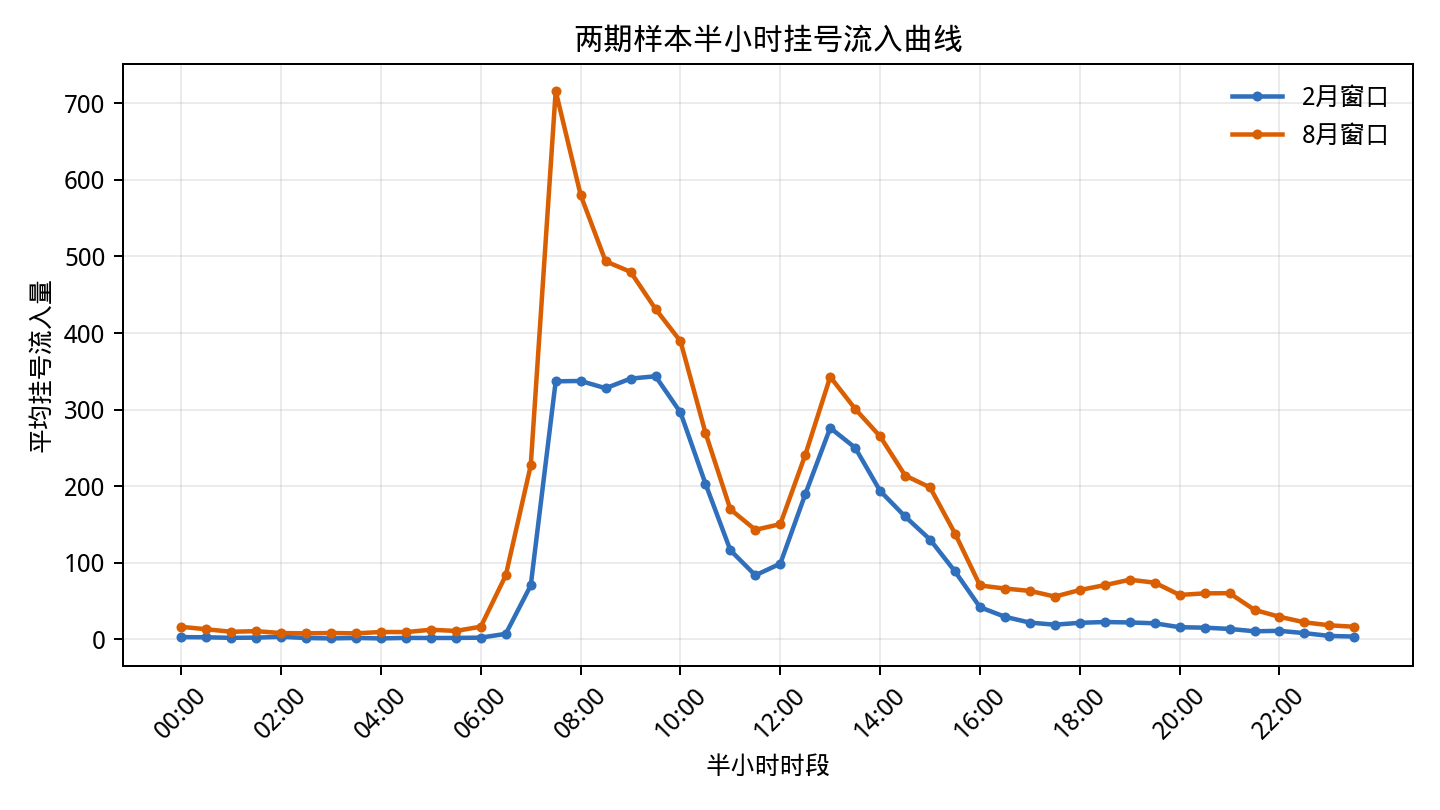
\includegraphics[width=0.86\textwidth,height=0.62\textheight,keepaspectratio]{arrival_profile.png}
  \vspace{0.4em}

  \Large 两期样本均呈现上午开诊前后的集中到达，8月窗口峰值更高
\end{frame}

\begin{frame}
  \bigidea{服务时长右偏与等待上移}
  \centering
  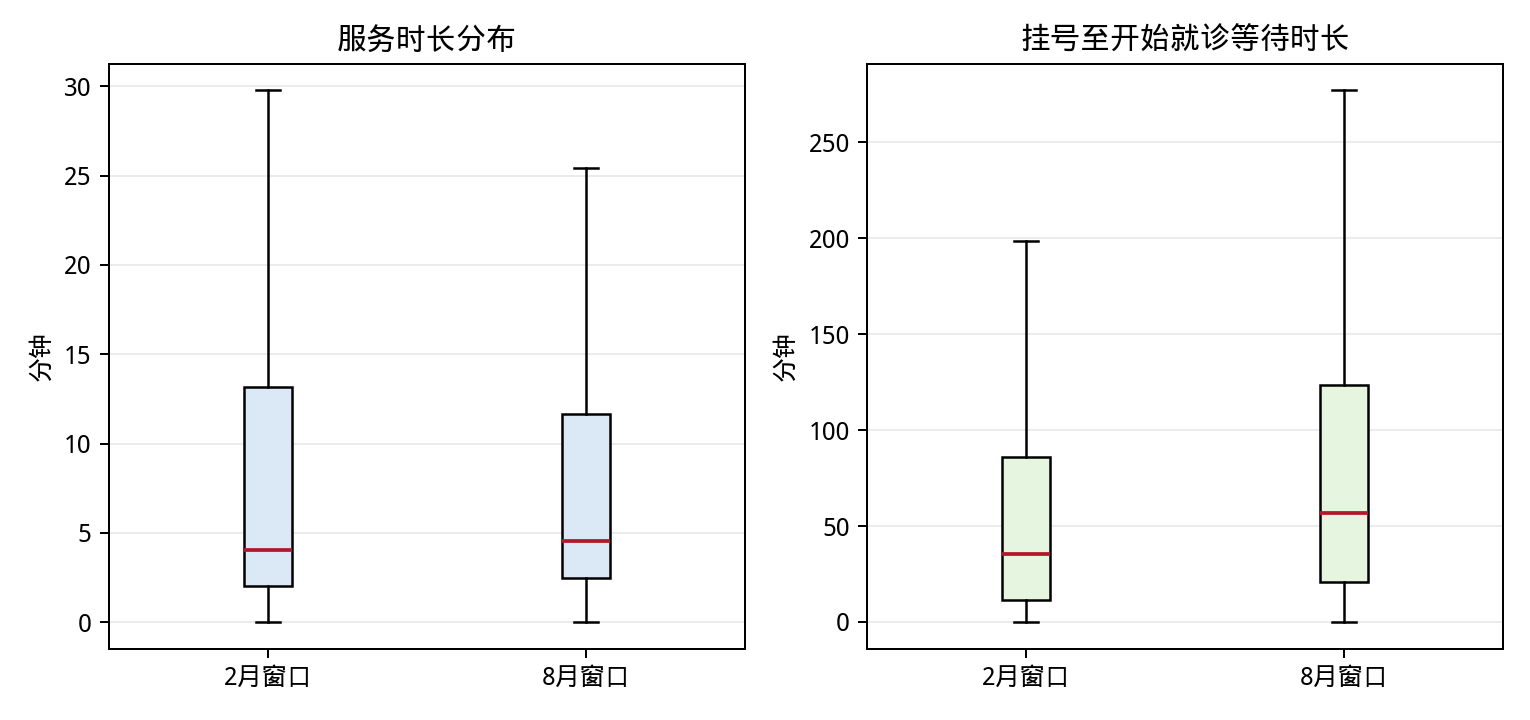
\includegraphics[width=0.86\textwidth,height=0.62\textheight,keepaspectratio]{service_wait_boxplot.png}
  \vspace{0.4em}

  \Large 服务时长分布相近，但8月等待时长整体上移
\end{frame}

\sectionpageframe{实证结果}

\begin{frame}
  \bigidea{策略输出构造}
  \begin{itemize}
    \item \Large 将每个医生--日期--时段状态代入确定性风险约束
    \item \Large Model 1 生成服务时长目标 $s^{(1)\star}$
    \item \Large Model 2 生成服务时长目标 $s^{(2)\star}$ 和预约开放目标 $u^{(2)\star}$
    \item \Large Model 3 进一步生成诊室层面的 $s_i^{(3)\star}$ 与 $u_i^{(3)\star}$
  \end{itemize}
\end{frame}

\begin{frame}
  \bigidea{反馈决策函数拟合结果}
  \centering
  \scriptsize
  \setlength{\tabcolsep}{3pt}
  \begin{tabular}{lllrrrr}
    \toprule
    模型 & 策略输出 & 输入状态 & 2月RMSE & 2月$R^2$ & 8月RMSE & 8月$R^2$ \\
    \midrule
    Model 1 & 服务时长 & $W$ & 2.741 & 0.404 & 2.917 & 0.384 \\
    Model 2 & 服务时长 & $W,B^{near},G^{near}$ & 2.865 & 0.458 & 3.026 & 0.423 \\
    Model 2 & 预约开放 & $W,B^{near},G^{near},R$ & 1.414 & 0.288 & 1.150 & 0.331 \\
    Model 3 & 服务时长 & $W,B^{near},G^{near},$系统压力 & 2.334 & 0.418 & 2.473 & 0.392 \\
    Model 3 & 预约开放 & $W,B^{near},G^{near},R,$系统状态 & 1.409 & 0.340 & 1.202 & 0.367 \\
    \bottomrule
  \end{tabular}
\end{frame}

\begin{frame}
  \bigidea{服务时长函数：预约簿状态有效}
  \begin{itemize}
    \item \Large Model 1 只使用排队工作量，2月和8月 $R^2$ 分别为 0.404 和 0.384
    \item \Large Model 2 加入近期已预约数量和剩余号源，$R^2$ 提升至 0.458 和 0.423
    \item \Large 说明服务速度决策不仅取决于眼前队列，也取决于即将到来的预约压力
  \end{itemize}
\end{frame}

\begin{frame}
  \bigidea{预约开放函数：系统状态有补充}
  \begin{itemize}
    \item \Large Model 2 预约开放函数 $R^2$ 为 0.288 和 0.331
    \item \Large Model 3 加入系统层状态后，$R^2$ 提升至 0.340 和 0.367
    \item \Large 多诊室压力和剩余号源信息，有助于解释后续窗口开放数量
    \item \Large 高压力状态下，开放策略以小规模、谨慎开放为主
  \end{itemize}
\end{frame}

\begin{frame}
  \bigidea{模型拟合表现比较}
  \centering
  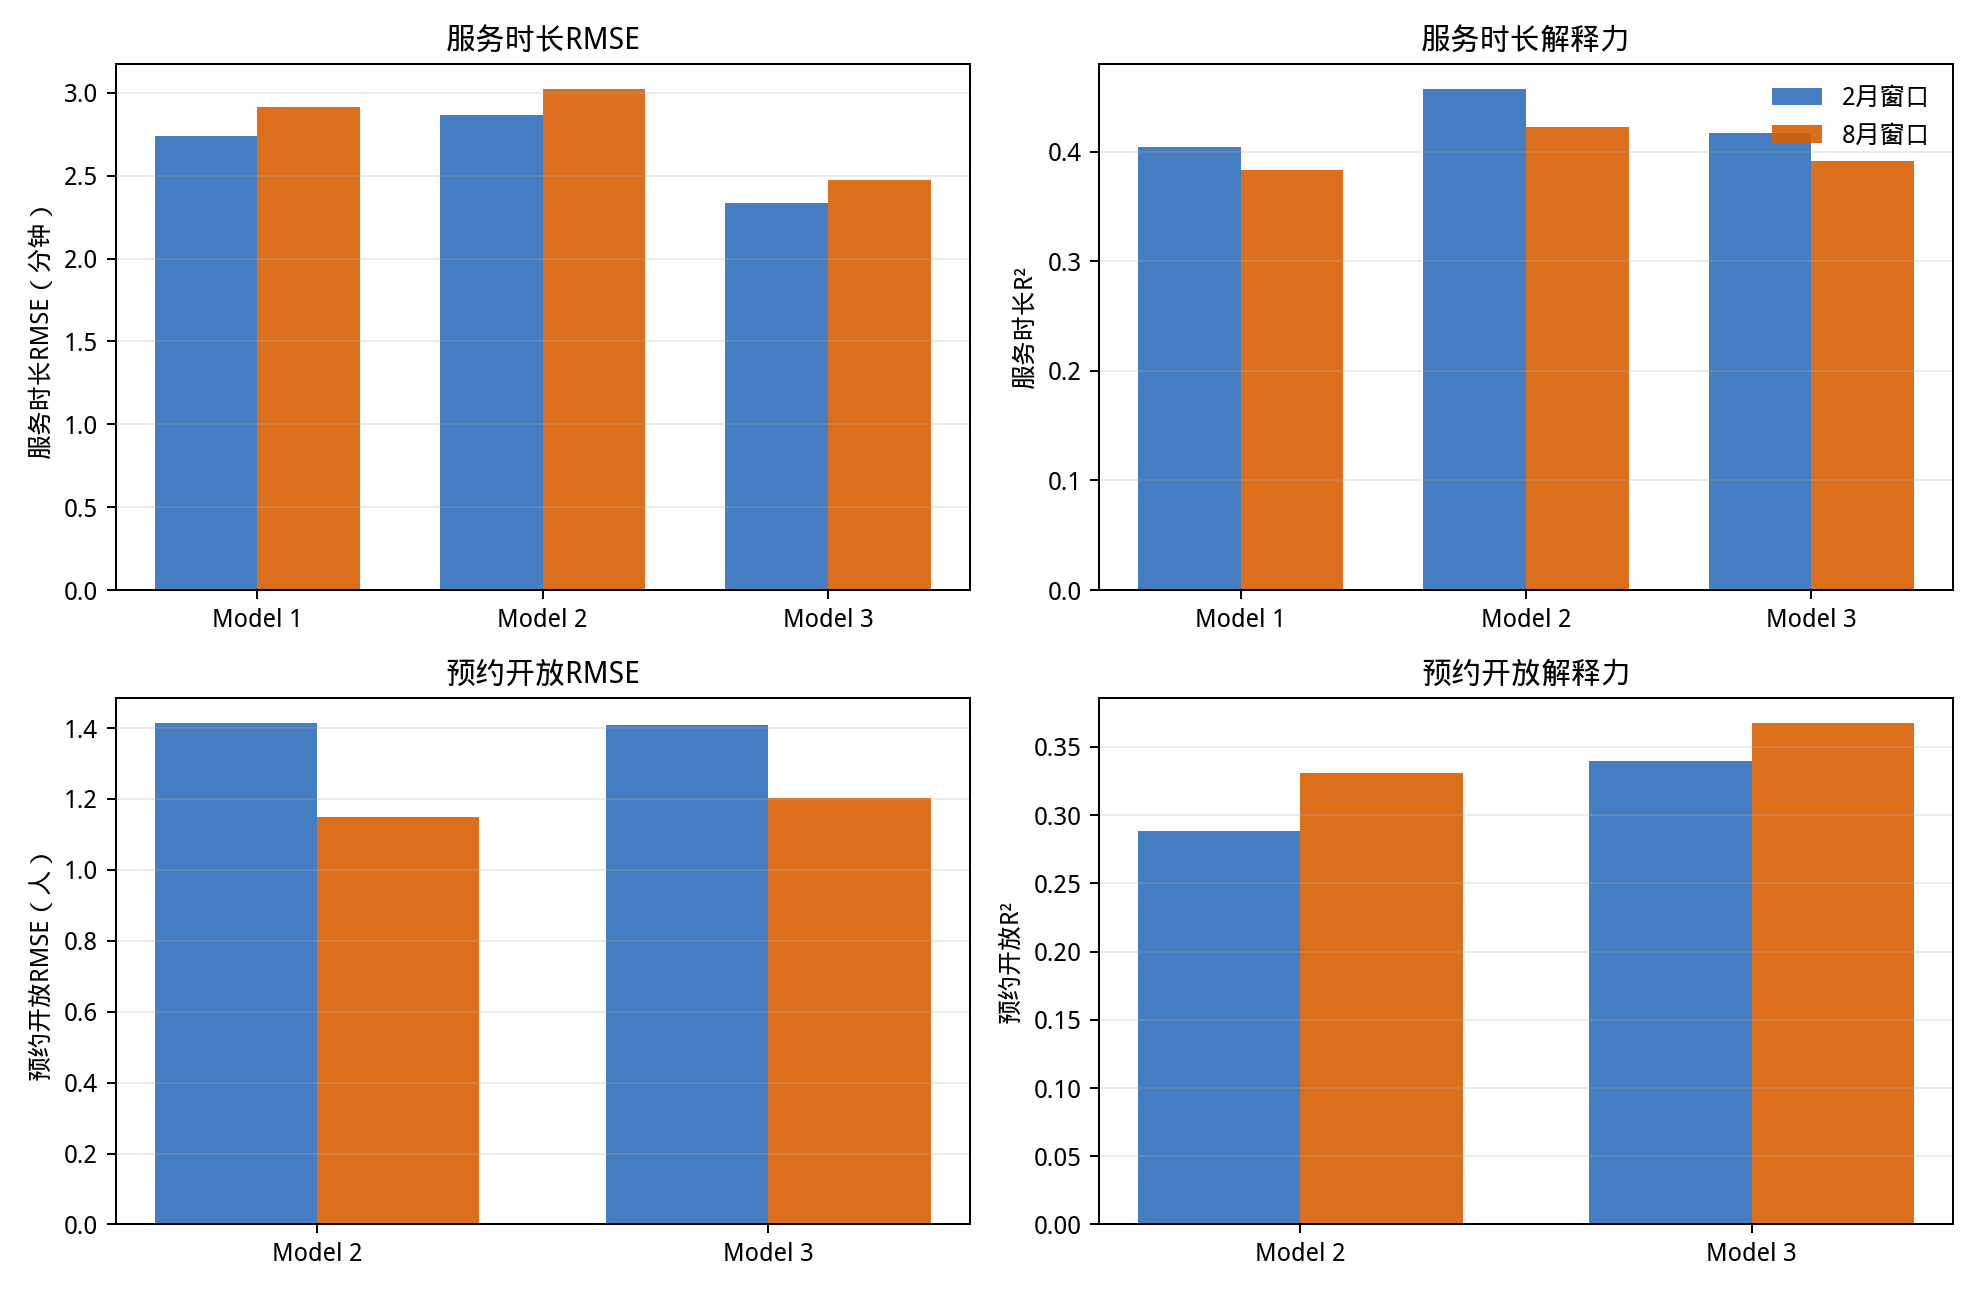
\includegraphics[width=0.88\textwidth,height=0.64\textheight,keepaspectratio]{model_function_comparison.png}
  \vspace{0.4em}

  \Large 两期窗口的误差与解释力保持在相近量级
\end{frame}

\begin{frame}
  \bigidea{反馈函数形态}
  \centering
  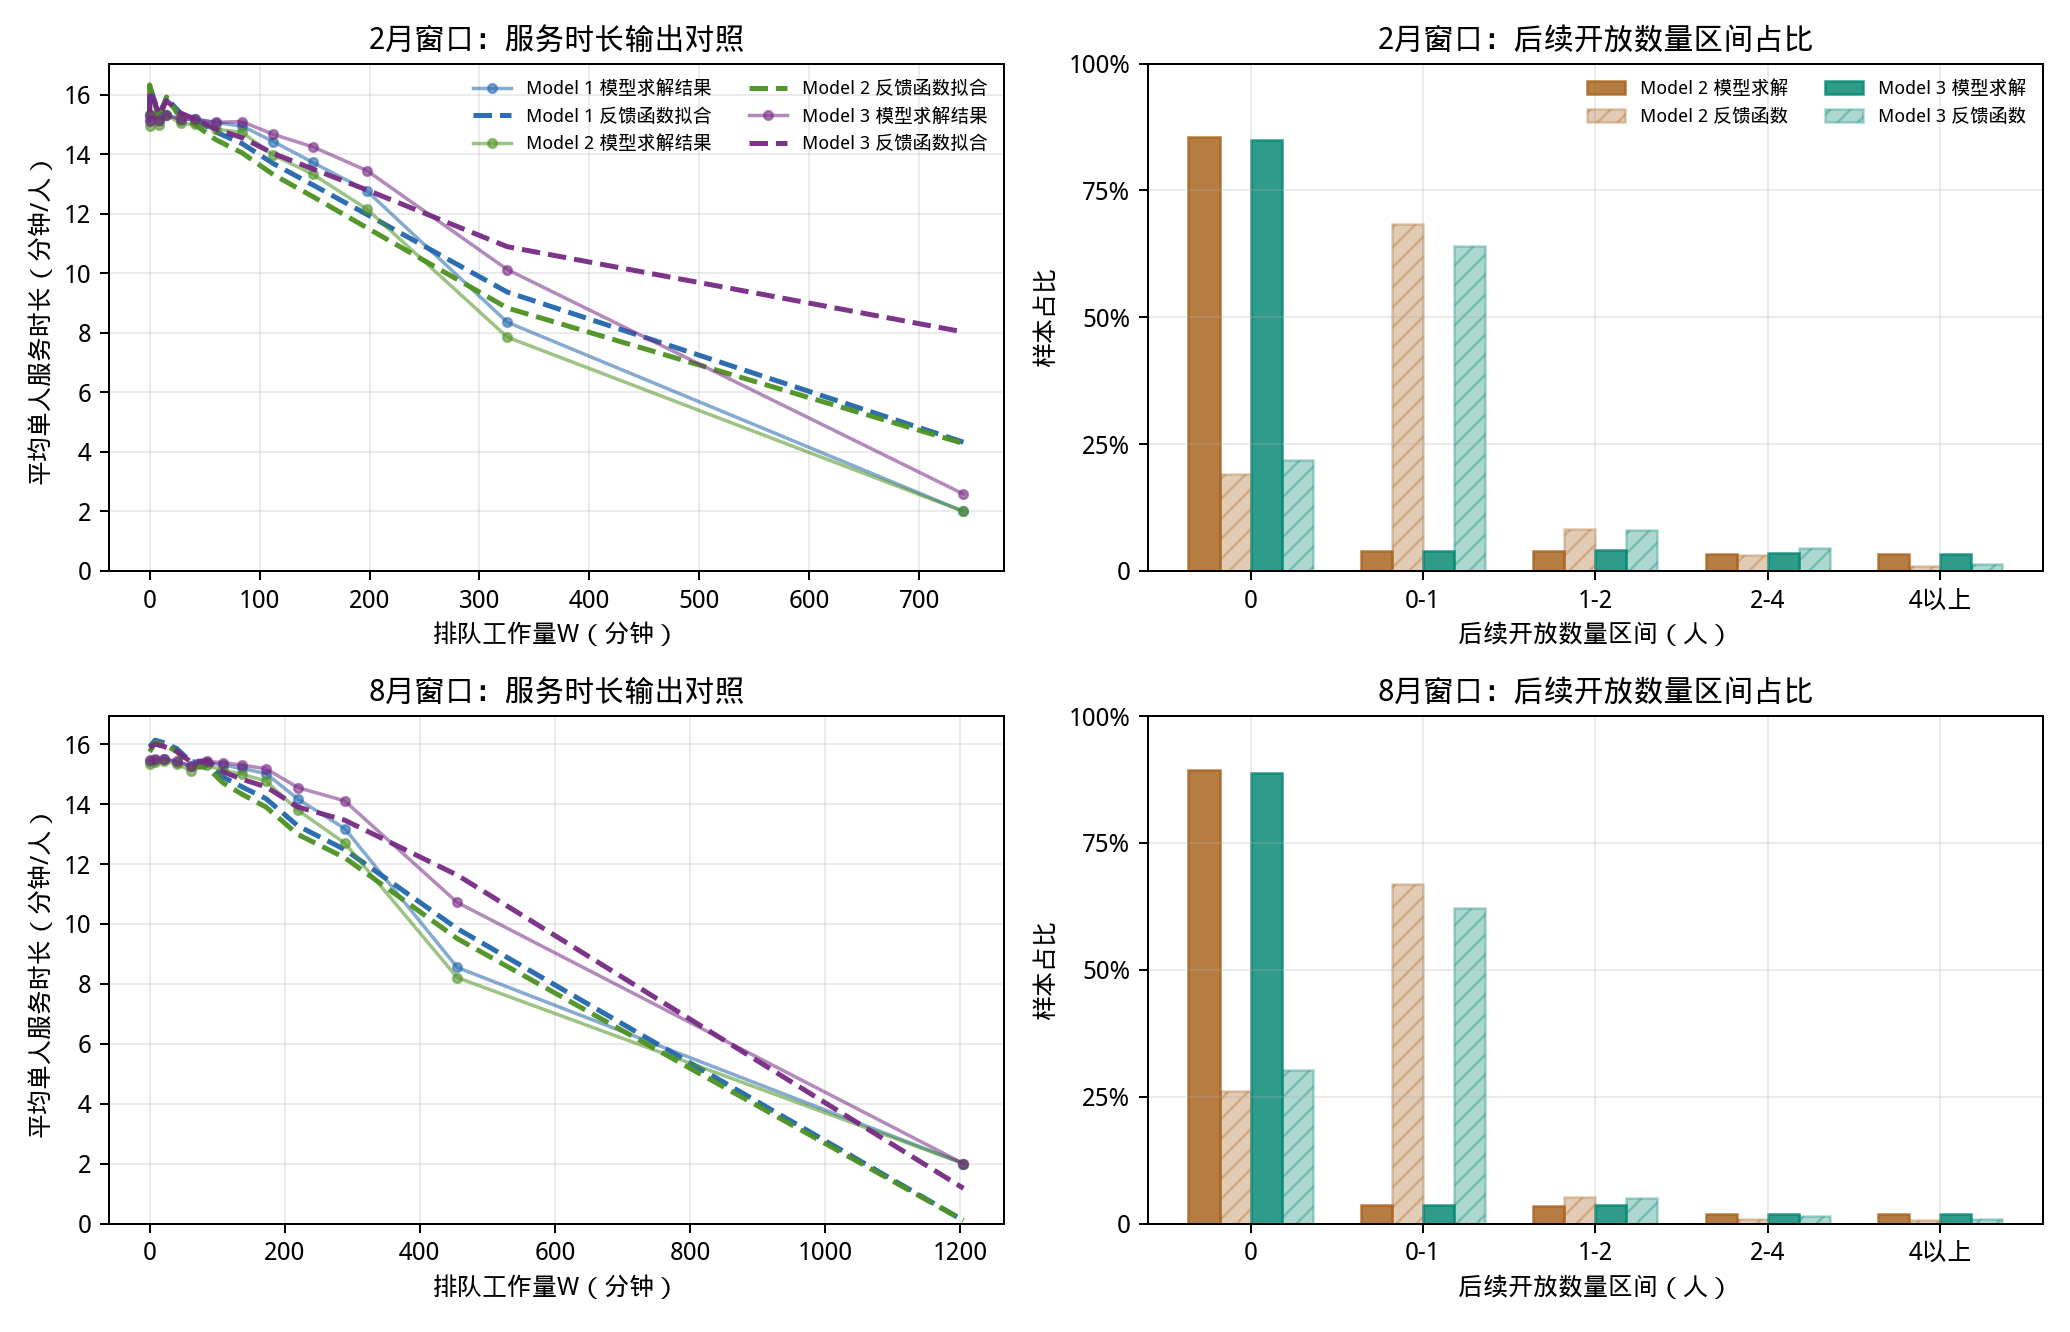
\includegraphics[width=0.88\textwidth,height=0.64\textheight,keepaspectratio]{feedback_fit.png}
  \vspace{0.4em}

  \Large 排队工作量上升时，模型倾向于压缩平均服务时长
\end{frame}

\sectionpageframe{结论}

\begin{frame}
  \bigidea{主要结论}
  \begin{itemize}
    \item \Large 门诊短时段流入存在明显过度离散，8月窗口等待压力更高
    \item \Large 服务时长分布右偏，少数长时患者对服务需求方差影响较大
    \item \Large 预约簿状态增强服务时长决策函数解释力
    \item \Large 系统层状态增强多诊室预约开放函数刻画能力
  \end{itemize}
\end{frame}

\begin{frame}
  \bigidea{管理含义}
  \begin{itemize}
    \item \Large 门诊调度不能只看平均等待，还应监控尾部压力
    \item \Large 高峰期服务加速存在边界，持续赶工会带来质量和职业风险
    \item \Large 预约开放应与当前排队、近期预约负荷和系统剩余能力联动
    \item \Large 模型可作为门诊调度看板中的策略提示模块
  \end{itemize}
\end{frame}

\begin{frame}
  \bigidea{不足与展望}
  \begin{itemize}
    \item \Large 样本来自两个14天窗口，后续可扩展到更长周期和更多科室
    \item \Large 预约请求变量由历史预约记录代理，仍可接入更直接的请求日志
    \item \Large 当前策略输出采用连续松弛，落地时需要加入取整和业务规则
    \item \Large 后续可进一步评估策略对患者等待、医生负荷和服务质量的实际影响
  \end{itemize}
\end{frame}

\begin{frame}[plain]
  \begin{center}
    \vfill
    {\Huge \bfseries 谢谢各位老师}

  \end{center}
\end{frame}

\end{document}
